When encountering the terminal for the first time one soon realises that some basic commands 
are needed to navigate the folders, edit, copy or delete files, etc ... 

For Windows users, you must abandon your preconceived (and totally arbitrary) ideas about the 
'C:' drive. Before hard drives even existed, the computer would have one or two floppy drives
and would reserve the A: and B: drive letters for them. Nowadays these devices are usually not installed 
in the computer anymore, but the labelling remains\footnote{\url{https://en.wikipedia.org/wiki/Drive_letter_assignment}}. 

The root of the file system is simply {\tt /}. Your 'home' is most likely in {\tt /home/your-family-name/}. Inside 
this you will find {\tt Documents}, {\tt Downloads}, etc ...

The basic set of commands is in fact not very large (Please also watch \url{https://youtu.be/6bMYzzrycV0}):


\begin{itemize}
%..............................
\item {\color{teal} \bf man}: 
Documentation in Linux is mostly available in the form of {\it man pages}.
They are usually written in the style of a reference manual and can be daunting at first.
They are usually:
the name, a compact formulation of the syntax (that can be scary for more complex programs),
a description about what the software actually is and does, 
examples (if you are lucky) and explanations of all the options mentioned above.
Typical use:
\begin{mdframed}[backgroundcolor=gray!10]
\begin{verbatim}
> man name-of-command-I-want-to-learn-about
\end{verbatim}
\end{mdframed}

%..............................
\item {\color{teal} \bf cd}: it stands for 'change directory' (i.e. change folder). 
Typical use:
\begin{mdframed}[backgroundcolor=gray!10]
\begin{verbatim}
> cd results 
\end{verbatim}
\end{mdframed}
where {\tt results} should be an existing folder. You can check this with:

%..............................
\item {\color{teal} \bf ls}: it stands for 'list'. This commands lists 
all files and folders 
Typical use:
\begin{mdframed}[backgroundcolor=gray!10]
\begin{verbatim}
> ls 
\end{verbatim}
\end{mdframed}
or 
\begin{mdframed}[backgroundcolor=gray!10]
\begin{verbatim}
> ls -la 
\end{verbatim}
\end{mdframed}
if you wish to have one item per line,
or 
\begin{mdframed}[backgroundcolor=gray!10]
\begin{verbatim}
> ls -l 
\end{verbatim}
\end{mdframed}
if you also want to see all files/folders starting with '.'
My preference goes to 
\begin{mdframed}[backgroundcolor=gray!10]
\begin{verbatim}
> ls -lhG 
\end{verbatim}
\end{mdframed}
Use the 'man' command to know what this does!

%..............................
\item {\color{teal} \bf mv}: it stands for 'move' but it has in fact a hidden functionality: rename.
If you type 
\begin{mdframed}[backgroundcolor=gray!10]
\begin{verbatim}
> mv garfield.txt odie.txt 
\end{verbatim}
\end{mdframed}
then the file {\filenamefont garfield.txt} has been renamed {\filenamefont odie.txt}
\footnote{\url{https://en.wikipedia.org/wiki/Odie} Obviously one cannot transform Garfield into 
Odie.}. 

You can move a file in a different folder as follows:
\begin{mdframed}[backgroundcolor=gray!10]
\begin{verbatim}
> mv garfield.txt ../myfolder/
\end{verbatim}
\end{mdframed}
This moves the file to a folder that is one level up. This will work only if the folder exists.
If you need to make a new folder, then use:
%..............................
\item {\color{teal} \bf mkdir}: it stands for 'make directory'. Typical usage
\begin{mdframed}[backgroundcolor=gray!10]
\begin{verbatim}
> mkdir res_123 
\end{verbatim}
\end{mdframed}
creates a folder named {\foldernamefont res\_123}. 


%..............................
\item {\color{teal} \bf rm}: it stands for 'remove'. Before we go any further: this command is dangerous. 
Unlike its counterpart based on selecting a file with a mouse and deleting it, rm does not send 
the file to the Trash folder (or Windows Recycle Bin). It simply deletes it forever. No turning back!
Typical usage
\begin{mdframed}[backgroundcolor=gray!10]
\begin{verbatim}
> rm myoldfile.txt
\end{verbatim}
\end{mdframed}
deletes the file. 
Note that by default, it does not remove directories. In order to remove a folder, one needs to 
type
\begin{mdframed}[backgroundcolor=gray!10]
\begin{verbatim}
> rm -r myoldfolder 
\end{verbatim}
\end{mdframed}
Unless you are an experienced user, never use {\tt rm} in conjunction with {\tt *} and/or in a recursive way.
If things go wrong, you will delete entire portions of your hard drive at best, or will destroy your operating system at worse.  


\item {\color{teal} \bf pwd}: it stands for 'print working directory'. If you are unsure of where
the current prompt of the terminal is, simply 
\begin{mdframed}[backgroundcolor=gray!10]
\begin{verbatim}
> pwd 
\end{verbatim}
\end{mdframed}
and it will return the full path, from the root to where the prompt is. 


\item {\color{teal} \bf du}: it stands for 'disk usage'. In this case always tag the -h option to it:
\begin{mdframed}[backgroundcolor=gray!10]
\begin{verbatim}
> du -h 
\end{verbatim}
\end{mdframed}
It will list the size of all folders in the folder the prompt is in. If you wish to know the size of an object
simply do 
\begin{mdframed}[backgroundcolor=gray!10]
\begin{verbatim}
> du -h file-or-folder 
\end{verbatim}
\end{mdframed}
The {\tt ls -lh} command would have told you as much, but for all files inside the folder.

\item {\color{teal} \bf grep}: searches for patterns in each file. Typical usage 
\begin{mdframed}[backgroundcolor=gray!10]
\begin{verbatim}
> grep linear *.tex 
\end{verbatim}
\end{mdframed}
This searches all occurrences of the word 'linear' in all .tex files. If you 
wish to look for this word in all files inside subfolders:
\begin{mdframed}[backgroundcolor=gray!10]
\begin{verbatim}
> grep -r linear .
\end{verbatim}
\end{mdframed}

\item {\color{teal} \bf more}: allows to visualise the content of an ascii\footnote{\url{https://en.wikipedia.org/wiki/ASCII}} file
inside the terminal without using a text editor. In other words, you can look into the file but not change its content.
\begin{mdframed}[backgroundcolor=gray!10]
\begin{verbatim}
> more interesting-file
\end{verbatim}
\end{mdframed}
 

\item {\color{teal} \bf top/htop}: allows to visualise which process is running on the computer and how much CPU and memory it takes.




\item {\color{teal} \bf wget}: it is a computer program that retrieves content from web servers. 
It is part of the GNU Project. Its name derives from "World Wide Web" and "get." 
It supports downloading via HTTP, HTTPS, and FTP.  
\begin{mdframed}[backgroundcolor=gray!10]
\begin{verbatim}
> wget address.of.file.online.on.server
\end{verbatim}
\end{mdframed}
See example of use in Section \ref{ss:1416wget}.


\item {\color{teal} \bf ssh}:  This command is necessary to connect to a remote computer from the terminal. 
By default most Linux computers run a client and server ssh program so that one can connect to 
any other computer if its address is known (as well as the username and password).
Here is how I connect to my shrek desktop computer:
\begin{mdframed}[backgroundcolor=gray!10]
\begin{verbatim}
> ssh shrek.geo.uu.nl -Y -l thieulot
\end{verbatim}
\end{mdframed}
The -Y option ensures that I have X11 support. If successful, the prompt of the terminal points
to the default folder on the remote machine and I can control the remote computer via the command line. 
Type exit to break the connection.

This is used to log in on remote servers like clusters where large calculations take place. 
 

\item {\color{teal} \bf sftp}: allows to get or put files on a remote computer via a secrured connection. By default, SFTP uses the SSH protocol to authenticate and establish a secure connection. Because of this, the same authentication methods are available that are present in SSH.
\begin{mdframed}[backgroundcolor=gray!10]
\begin{verbatim}
> sftp garfield@remote.univ.nl 
\end{verbatim}
\end{mdframed}
This will prompt for the password of the remote machine associated to user garfield.
If succesful the prompt in the terminal then points to the default folder on the remote computer.
Once connected simply type exit to break the connection. 
All shell commands are available: pwd, ls, cd, etc ...
you can list the contents of the current directory on the local machine using {\tt lls}.
If we want to download files from our remote host, you can do so using the get command:
\begin{mdframed}[backgroundcolor=gray!10]
\begin{verbatim}
> get remotefile 
\end{verbatim}
\end{mdframed}
If you wish to download an entire folder, simply use 
\begin{mdframed}[backgroundcolor=gray!10]
\begin{verbatim}
> get -r remotefolder 
\end{verbatim}
\end{mdframed}
Conversely, you can transfer files from your local machine onto the remote one:
\begin{mdframed}[backgroundcolor=gray!10]
\begin{verbatim}
> put remotefile 
\end{verbatim}
\end{mdframed}


 



\item {\color{teal} \bf scp}:   to do 



\end{itemize} 


\vspace{1cm}

In what follows I list a few 'tricks' which I find useful or just can never remember:

\begin{itemize}
\item How to convert files in batch 

\begin{mdframed}[backgroundcolor=gray!10]
\begin{verbatim}
> convert '*.png' converted_%04d.jpg
\end{verbatim}
\end{mdframed}

\item How to Remove unwanted empty lines in a file with vi(m)\\
Use either of the following commands to delete all empty lines: 
\begin{mdframed}[backgroundcolor=gray!10]
\begin{verbatim}
:g/^$/d
:v/./d
\end{verbatim}
\end{mdframed}
If you want to delete all lines that are empty or that contain only whitespace 
characters (spaces, tabs), use either of: 
\begin{mdframed}[backgroundcolor=gray!10]
\begin{verbatim}
:g/^\s*$/d
:v/\S/d
\end{verbatim}
\end{mdframed}

\item How to find LAPACK
\begin{mdframed}[backgroundcolor=gray!10]
\begin{verbatim}
## BLAS: /usr/lib/x86_64-linux-gnu/blas/libblas.so.3.7.1
## LAPACK: /usr/lib/x86_64-linux-gnu/lapack/liblapack.so.3.7.1
\end{verbatim}
\end{mdframed}

\item How to apt-get MUMPS

\begin{mdframed}[backgroundcolor=gray!10]
\begin{verbatim}
> sudo apt-get install libmumps-seq-dev
\end{verbatim}
\end{mdframed}

\item How to remove a big file wrongly committed

\begin{mdframed}[backgroundcolor=gray!10]
\begin{verbatim}
> git filter-branch --tree-filter 'rm -rf path/to/your/file' HEAD
> git push
\end{verbatim}
\end{mdframed}

\item How to check your disk usage (ubuntu)\\

Disk Usage Analyzer (aka Baobab) is a graphical, menu-driven viewer 
that you can use to view and monitor your disk usage and folder structure. 
It is part of every GNOME desktop.

\begin{mdframed}[backgroundcolor=gray!10]
\begin{verbatim}
> baobab
\end{verbatim}
\end{mdframed}

\begin{center}
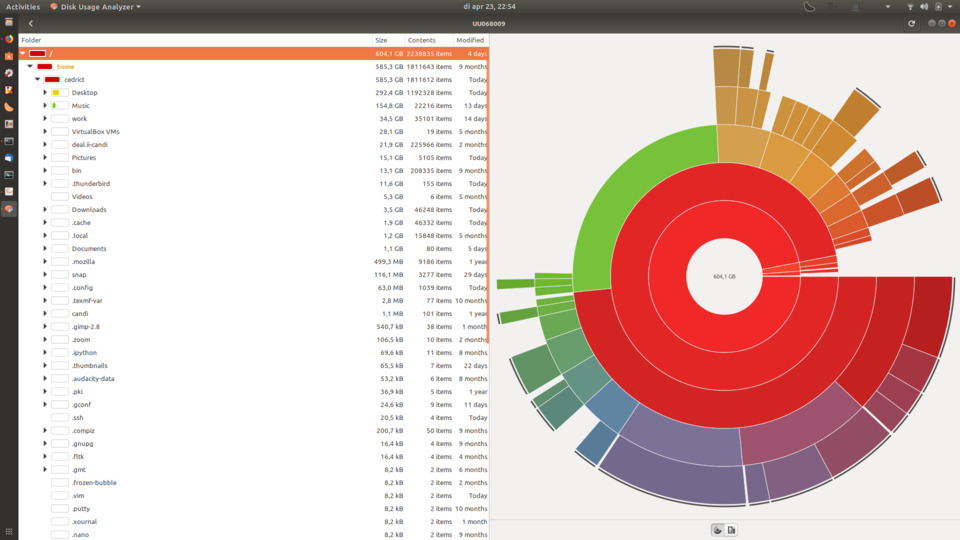
\includegraphics[width=7cm]{images/baobab}
\end{center}


\item How to convert images into another format in the command line

\begin{mdframed}[backgroundcolor=gray!10]
\begin{verbatim}
> convert file.png file.jpg
\end{verbatim}
\end{mdframed}

You can also resize on the fly:

\begin{mdframed}[backgroundcolor=gray!10]
\begin{verbatim}
> convert -resize 70% file.png file.jpg
\end{verbatim}
\end{mdframed}


\item How to compress files:
tar is used to pack files into an archive without zipping them. 
This enables easy attaching to email, or to sending across the internet without the computer having
to start a new transfer for every file. 
Also it ensures everything belong to a certain package stays together.
Optionally it can be used to zip files.
Let us have an example of three files; {\it a.txt, b.py} and {\it c.dat}
These can be packed together with

\begin{mdframed}[backgroundcolor=gray!10]
\begin{verbatim}
> tar -cf allFiles.tar *
\end{verbatim}
\end{mdframed}

c stands for {\it compress} and f for {\it file}, as can be seen in the manpage of tar.
It can similarly be extracted using the command:

\begin{mdframed}[backgroundcolor=gray!10]
\begin{verbatim}
> tar -xf allFiles.tar *
\end{verbatim}
\end{mdframed}

to recover three original files.

Additionally, it is possible to zip them as well, by adding a z to the options. 
The default extension then becomes {\it tgz}:

\begin{mdframed}[backgroundcolor=gray!10]
\begin{verbatim}
> tar -czf allFiles.tgz *
> tar -xzf allFiles.tgz *
\end{verbatim}
\end{mdframed}



\end{itemize}

